\subsubsection{\stid{2.11} Argobots: Flexible, High-Performance Lightweight Threading }

\paragraph{Overview}

Efficiently supporting massive on-node parallelism demands highly
flexible and lightweight threading and tasking runtimes. At the
same time, existing lightweight abstractions have shortcomings while
delivering generality and specialization.  Our group at Argonne
developed a lightweight, low-level threading and tasking framework,
called Argobots.  The key focus areas of this project are: (1) To
provide a framework that offers powerful capabilities for users to
allow efficient translation of high-level abstractions to low-level
implementations. (2) To provide interoperability with other
programming systems such as OpenMP and MPI as well as with other
software components (e.g., I/O services). (3) To provide a programming
framework that manages hardware resources more efficiently and reduce
interference with colocated applications.

\paragraph{Key Challenges}

Several user-level threading and tasking models have been proposed in
the past to address the shortcomings of OS-level threads, primarily
with respect to cost and flexibility. Their lightweight nature and
flexible generic interface play an important role at managing
efficiently the massive concurrency expected at the Exascale level.
Existing user-level threading and tasking models, however, are either
too specific to applications or architectures or are not powerful or
flexible. Existing runtimes tailored for generic use \cite{GNUPth,
PLDI97_Taura, COSET05_Thibault, COB14_Nakashima, MTAAP08_Wheeler,
PPoPP99_Taura, SenSys06_Dunkels, TBB1, EuroPar08_Perache} are suitable
as common frameworks to facilitate portability and interoperability
but offer insufficient flexibility to efficiently capture higher-level
abstractions, while specialized runtimes \cite{ATC02_Adya,
SolarisThreads, SOSP03_von_Behren, StateThreads, PLDI07_Li,
MTAAP09_Porterfield, WMPP05_Cuvillo, IntelOMP, Nanos++, LCPC96_Kale,
PACT14_Treichler} are tailored to specific environment.

\paragraph{Solution Strategy}

Argobots offers a carefully designed execution model that balances
generality of functionality with providing a rich set of controls to
allow specialization by end users or high-level programming models
\cite{seo2018}.  Delivering high performance in Argobots while
providing a rich set of capabilities is achieved by heavily optimizing
critical paths as well as by exposing configuration knobs and a rich
API, which allow users to trim unnecessary costs. Furthermore,
Argobots honors high degrees of expressibility through the following
three key aspects:

\begin{enumerate}

\item Capturing the requirements of different \emph{work units}, which
are the most basic manageable entities. Work units that require
private stacks and context-saving capabilities, referred to as
\textit{user-level threads} (ULTs, also called \textit{coroutines} or
\textit{fibers}), are fully fledged threads usable in any context.
\emph{Tasklets} do not require private stacks. They are more
lightweight than ULTs because they do not incur context saving and
stack management overheads.  Tasklets, however, are restrictive; they
can be executed only as atomic work units that run to completion
without context switching.

\item Exposing hardware computational units through \emph{execution
streams} (ESs) as OS-level threads to execute work units. Unlike
existing generic runtimes, ESs are exposed to and manageable by users.

\item Allowing full control over \emph{work unit management}.  Users
can freely manage \emph{scheduling} and mapping of work units to ESs
through \emph{thread pool} management, and thus achieving the desired
behavior. Figure~\ref{fig:sollve-argobots} illustrates the various
building blocks in the Argobots framework and the interactions between
them to build a hypothetical system.

\end{enumerate}

\begin{figure}[htb]
  \centering
  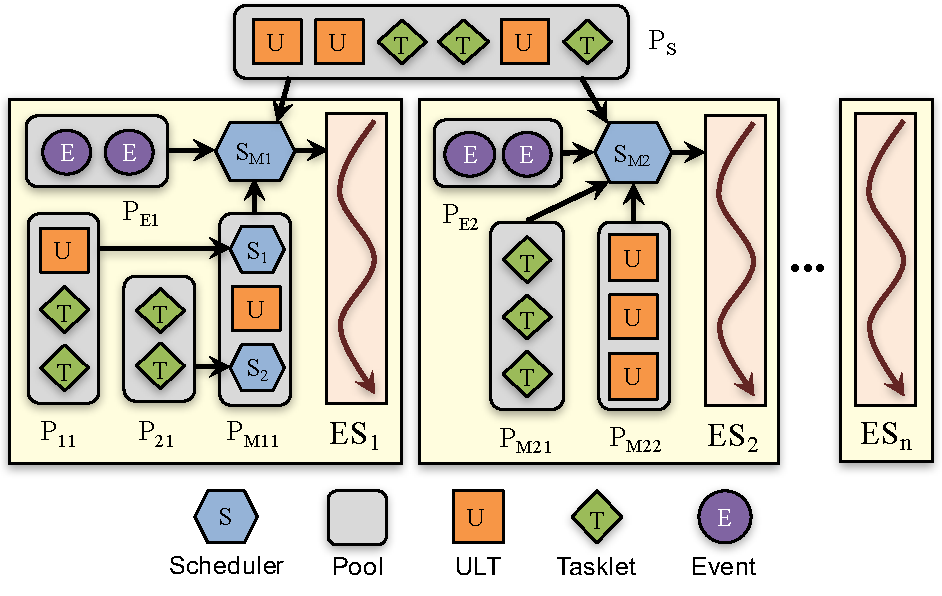
\includegraphics[height=3in]{projects/2.3.2-Tools/2.3.2.11-SOLLVE/SOLLVE-ARGOBOTS.pdf}
  \caption{\label{fig:sollve-argobots}Argobots execution model}
\end{figure}

\paragraph{Recent Progress}

Integration with other runtime systems is fundamentally important for
the Argobots project. BOLT, an LLVM OpenMP runtime over Argobots, is
one of the most successful parallel programming systems using
Argobots. Thread scheduling mechanism tailored to the OpenMP
specification plays a key role in efficient and effective exploitation
of nested parallelism in BOLT. As a result, BOLT outperforms existing
OS-level thread-based and ULT-based OpenMP runtime
systems~\cite{BOLT}. This showcases the importance of exposing
low-level threading functionalities including customizable thread
schedulers and thread pool operations. The Argobots project continues
to improve interoperability with communication layers such as MPI
runtimes (e.g., MPICH and Open MPI) and Mercury RPC; Argobots benefit
these communication libraries  by lightweight user-level context
switch and flexible user-level scheduling. I/O service is one of the
most important application areas for Argobots. Intel DAOS, a high
performance storage system developed by Intel, uses Argobots to
efficiently handle asynchronous I/O messages. We implemented several
features and performed optimizations that are demanded by these key
projects, including several debugging functionalities in Argobots.

Overheads of thread creation and scheduling highly impact the
performance of applications and runtimes parallelized with Argobots.
Our study has proven that a \textit{dynamic promotion technique},
which initially creates ULTs with minimum features and lazily promotes
threads when an independent context gets required, are effective in
the scenario where chances of suspension are low~\cite{iwasaki2018}.
In addition to support of x86/64 architectures, we extended this
technique to various CPU architectures that are commonly seen in HPC:
POWER and ARM. One of our recent efforts is improvement of testing
with continuation integration by increasing test cases, testing
compilers, and architectures in order to deliver a stable and
well-tested implementation of Argobots.

\paragraph{Next Steps}

Argobots continues to implement new features and optimizations for
application needs, while our substantial efforts will be made to
promote integration and composition with other systems. Another key
aspect is educating users and growing the user base of Argobots. Our
major ongoing and planned steps are as follows.

\begin{enumerate}

\item Further integration with communication layers including MPI
runtimes and Mercury RPC. Particularly, we continue to collaborate
with MPICH and Open MPI developers to make their Argobots
interoperability layers more scalable and stable.

\item Enhanced interoperability of multiple Argobots-aware components.
As more and more software components use Argobots, managing resources
in Argobots across multiple Argobots-aware software stacks gets
challenging.  For example, blindly creating ESs can incur
oversubscription of OS-level threads, which significantly lowers
performance. To address this issue, we are investigating an approach
that virtualizes the execution stream layer in Argobots.

\item Provides tutorials for users and grows the community. The user
community is precious to get feedback and bug reports and stabilize
developments as well as expand the Argobots ecosystem. As our tutorial
on Argobots at PACT '19 was successful, we plan to have another at
PPoPP '20.

\end{enumerate}
